\subsection*{Introduction}


Nowadays \emph{Computer Vision} and \emph{Image Processing (IP)} are omnipresent in the day-to-day
life of the people. It is present each time we pass by a CCTV camera, each time we go to the hospital do an MRI, each
time we drive our car and pass in front of a speed camera and each time we use our computer, smartphone or tablet. It
cannot be avoided it anymore. The systems using this technology are sometimes simple and, sometimes, more complex. Also,
the usage made of this technology has many purposes such as space observation, medical, quality of life improvement,
surveillance, control, autonomous system, etc. Henceforth, \emph{Image Processing} has a wide range of research and
despite having a mass of previous of work already contributed to, there are still a lot to explore.

Let us take the example of a modern smartphone application which provides facial recognition in order to recognize
people whom are featuring inside a photo. To provide an accurate result, this application will have to do a lot of
different processing through several steps. In addition, there are a lot of variables to handle. We can list (non
exhaustively) the weather, the light exposition, the resolution, the orientation, the number of person, the localization
of the person, the distinction between humans and objects/animals, etc. All of these elements needs to be carefully
handled in order to finally recognize the person(s) inside the photo. What the application does not tell you is the
complexity of the image processing pipeline behind the scene that, most of the time, cannot even be executed in its
entirety on one's device (smartphone, tablet, \ldots). Indeed, image processing is costly in computing resources and
would not meet the time requirement desired by the user if the entire pipeline was executed on the device. Furthermore,
for the final part which is ``recognize the person on the photo'', the application needs to feed the pre-processed photo
to a neural network trained beforehand through deep learning techniques in order to give an accurate response. There
exists technologies capable of embedding neural network into mobile phone such as
MobileNets~\parencite{howard.2017.mobilenets}, but it remains limited in terms of operational capabilities. It can
detect a human being inside a photo but not give the answer about whom this human being is for instance. That is why,
accurate neural network system usually are abstracted away in cloud technologies making them available only via
Internet. When uploading his image, the user does not imagine the amount of technologies and computing power that will
be used to find who appear on the photo.

We now understand that in order to build applications that interact with photos or videos nowadays, we need to be able
to do accurate, fast and scalable image processing on a multitude of devices (smartphone, tablet, \ldots). In order to
achieve this goal, image processing practitioners needs to have two kinds of tools at their disposal. The first is the
prototyping environment, a toolbox which allow the practitioner to develop, test and improve its application logic. The
second one is the production environment which deploys the viable version of the application that was developed by the
practitioner. Both environment may not have the same needs. On one hand, the prototyping environment usually requires to
have a fast feedback loop for testing, an availability of state-of-the-art algorithms and existing software. This way
the practitioner can easily build on top of them and be fast enough so that he does not wait a long time to get the
results when testing many prototypes. On the other hand, the production environment must be stable, resilient, fast and
scalable.

When looking at standards in the industry nowadays, we notice that the \emph{Python} programming language is the main
choice for prototyping. However, Python may not be suitable to push a viable prototype in production with minimal
changes afterwards. We find it non-ideal that the practitioner cannot take advantages of many optimization
opportunities, both in terms of algorithm efficiency and better hardware usage, when proceeding this way. It would be
much more efficient to have basic low level building blocks that can be adapted to fit as mush use cases as possible.
This way, the practitioner can easily build on top of them when designing its application. We distinguish two kinds of
use cases. The first one is about the multiplicity of types or algorithms the practitioner is facing. The second one is
about the diversity of hardware the practitioner may want to run his program. The goal is to have building blocks that
can be intelligent enough to take advantage of many optimization opportunities, with regard to both input data
types/algorithms and target hardware. Then the practitioner would have an important performance improvement, by default,
without specifically tweaking his application. As such, the concept of genericity was introduced. It aims at providing a
common ground about how an image should behave when passed to basic algorithms needed for complex applications. This
way, in theory, one only needs to write the algorithm once for it to work with any given kind of image.

In the end, it is often known that there is a rule of three about genericity, efficiency and ease of use. The rule
states that one can only have two of those items by sacrificing the third one. If one wants to be generic and efficient,
then the naive solution will be very complex to use with lots of parameters. If one wants a solution to be generic and
easy to use, then it will be not very efficient by default. Finally, If one wants a solution to be easy to use and
efficient then it will not be very generic. To illustrate this rule, we can find examples among existing libraries. A
notably generic and efficient library in C++ is Boost~\parencite{boost.2021}: it is also notably known to be hard to
use. Components such as Boost.Graph, Boost.Fusion or Boost.Spirit are hard to use. Also, a library which is generic and
easy to use is the Json parser written by Niels Lohmann~\parencite{nlohmann.2021.json} it strives to handle every use
case while remaining very easy to integrate and to use in user code (syntax really close to native Json in C++ code by
providing DSL Domain Specific Language)~\parencite{deursen.2000.DSL} to parse C++ constructs into JSON). However, this
has a cost and the parser is slower than Json parser optimized for speed such as
simdjson~\parencite{lemire.2021.simdjson} whose aim is to ``parse gigabytes of JSON per second''. Finally, there are
plenty of example of user-friendly and efficient code which is not generic. We can cite
Scikit-image~\parencite{vanderwalt.2014.skimage} and OpenCV~\parencite{bradski.2000.opencv} that are easy to use and
efficient (lot of handwritten SIMD/GPU code) but not generic due to the design choices.

In this thesis, we chose to work on an image processing library through continuing the work on
Pylene~\parencite{carlinet.2018.pylena}. But only working at library level would restrict the usability of our work and
thus its impact. That is why we aim to reach prototyping users through providing a package that can be used in dynamic
language such as Python without sacrificing efficiency. In particular, we aim to be useable in a Jupyter notebook. It is
a very important goal for us to reach a usability able to permeate into the educational side which is a strength of
Python. In this library, we demonstrate how to achieve genericity and efficiency while remaining easy to use all at the
same time. In doing so, we are endeavoring to breakthrough the rule previously cited. The scope of this library is
limited to mathematical morphology~\parencite{najman.2013.mathematical,geraud.2010.book} and to the provision of very
versatile image types. We leverage the modern C++ language and its many new features related to genericity and
performance to breakthrough this rule in the image processing area. Finally, we attempt, to bring low level tools and
concepts from the static world to the high level and dynamic prototyping world for a better diffusion and ease of use,
thanks to a bridge between those two worlds.

With this philosophy in mind, this manuscript aims at presenting our thesis work related to the C++ language applied to
the Image Processing domain. It is organized as followed:

\paragraph{Generic Programming (genericity)} This chapter presents a state-of-the-art overview about the notion of
genericity. We explain its origin, how it has evolved (especially within the C++ language), what issues it is solving,
what issues it is creating. We explain why image processing and genericity work well together. Finally, we tour around
existing facilities that allows genericity (intrinsically restricted to compiled language) to exists in the dynamic
world (with interpreted languages such as Python).

\paragraph{Taxonomy for Image Processing: Image types and Algorithms} This chapter presents our first contribution in
the image processing area which is a comprehensive work consisting in the the taxonomy of different images families as
well of different algorithms families. This chapter explains, among others, the notion of concept and how it applies to
the image processing domain. We explain how to extract a concept from existing code, how to leverage it to make code
more efficient and readable. We finally offer our take in the form of a collection of concepts related to image
processing area.

\paragraph{Images Views} This chapter presents our second contribution which is a generalization of the concept of View
(from the C++ language, the work on ranges~\parencite{niebler.2018.ranges}) to images. This allows the creation of
lightweight, cheap-to-copy images. It also enables a much simpler way to design image processing pipeline by chaining
operations directly in the code in an intuitive way. Ranges are the cement of new designs to ease the use of image into
algorithms which can further extend their generic behavior. Finally, we discuss the concept of lazy evaluation and the
impacts of views on performance.

\paragraph{A bridge between the static world and the dynamic world} This chapter presents our third contribution which
is a way to grant access to the generic facilities of a compiled language (such as C++) to a dynamic language (such as
Python) to ease the gap crossing between the prototyping phase and the production phase. Indeed, it is really not
obvious to be able to conciliate generic code from C++ whose genericity is resolved at compilation-time (we call this
the ``static world''), and dynamic code from Python which rely on pre-compiled package binaries (we call this the
``dynamic world''), to achieve an efficient communication between the dynamic code and the library. We also cannot ask
of the user to provide and use a compiler each time he wants to use our library from Python. In this chapter, we discuss
what are the existing solutions that can be considered as well as their \pros and \cons. We then discuss how we designed
a hybrid solution to make the bridge between the static world and the dynamic world.


\subsection*{Generic programming (genericity)}


In natural language we say that something is generic when it can fit several purposes at once while being decently
efficient. For instance, a computer is a generic tool that allows one to write documents, access emails, browse
Internet, play video games, watch movies, read e-books etc. In programming, we will say that a tool is generic when it
can fit several purposes. For instance, the gcc compiler can compile several programming languages (C, C++, Objective-C,
Objective-C++, Fortran, Ada, D, Go, and BRIG (HSAIL)) as well as target several architectures (IA-32 (x86), x86--64,
ARM, SPARC, etc.). Henceforth, we can say that gcc is a generic compiler. At this point it is important to note that
even though a tool is deemed generic, there is a scope on what the tool can do and what the tool cannot do. A compiler
despite supporting many languages and architectures, will not be able to make a phone call or a coffee. As such it is
important to note that genericity is an aspect that qualifies something. This chapter studies the generic aspects
related to libraries and programming languages.

This thesis voluntary leaves out the generic aspect related to the target architecture. Indeed, being able to write
and/or generate code that is able to run on a large array of different hardware architecture is a field of research on
its own and is not the main focus of this thesis. It is also known as \emph{heterogeneous computing}. Instead, we will
focus on the aspects related to genericity at a library level and at a programming language level.

\paragraph{Genericity within libraries} It is described by the cardinality of how many use-cases it can handle.
Libraries always provides their own data structures, to represent and to give a meaning to the data the user wants to
process, as well as algorithms to process those data and provide different type of results. A library will be then
labeled as \emph{generic}~\parencite{musser.1994.algorithm} when (i) its data structures allow the user to express
himself fully with no limitation and when (ii) its algorithm bank is large enough to do anything the user would want to
do with its data. In reality such a library does not exist and there are always limitations. Studying those limitations
and what reasons motivate them is the key to understand how to surpass them in the future, by developing new hardware
and/or software support for new features enabling more genericity.

\paragraph{Genericity within programming languages} It is described by the ability of the language to execute the same
code over a large amount of data structures~\parencite{dehnert.1998.fundamentals}, be they native (char, int, \ldots) or
user defined. It is nowadays primordial for a programming language to be able to do so. Indeed, in a world where
Information Technologies are everywhere, the amount of code written by software developers is staggering. And with it so
is the amount of bugs and security vulnerabilities. Being able to natively have a programming language that enables to
do \emph{more} by writing \emph{less} mathematically results in a reduced development and maintenance cost. Programming
languages offers many ways to achieve genericity which is dependent of the language intrinsic specificities: compiled or
interpreted, native or emulated, etc.

Before delving into the specifics of what genericity implies for libraries and programming languages, let us introduce
some vocabulary for the sake of comprehension. First is the notion of \emph{type}. A \emph{type} (or \emph{data type})
is an attribute of data which tells the compiler or interpreter how the programmer intends to use the data. Most
programming language support basic data types (also called primitive types) such as integer numbers, floating point
numbers, boolean and characters (ASCII, Unicode, etc.). This data attribute defines the operations that can be performed
on the data, the meaning of the data and the size of the data in memory (the data can then be stored on the heap, stack,
etc.). A data type provides a set of values from which an expression (\ie variable, function, etc.) may take those
values. Among programming language, we can distinguish those who are dynamically types and those that are statically
typed. Statically typed languages are those whose variables are declared holding a specific type. This variable cannot
hold data from another type in the scope it is declared. Statically typed programming languages are Ada, C, C++, Java,
Rust, Go, Scala. Dynamically types languages are those whose variables can be reassigned with a value of different type
from the one it was initially declared to hold. The variable type is then dynamically changed to fit the new value it is
holding. Dynamically typed programming languages are PHP, Python, JavaScript, Perl.

The consequence of being able to tell which type a variable is holding at all time (statically-typed language) is
two-fold. For the developer, it is easier to reason about code and to spot bugs. For the compiler, it is possible to
generate optimized binary code specific to this data type (vectorization, etc.). The consequence of being able to morph
the type a variable can hold at runtime is mainly to serve prototyping purpose. When tweaking a Jupyter notebook, it is
much appreciated not to be limited to a single type for each variable to be able to iterate on the prototype much
faster.

In image processing, an image \(Im\) is defined on a domain \(\mathcal{D}\) (which contains points) by the relation
\(\forall x \in \mathcal{D}, y = Im(x)\) where \(y\) is the value of the image \(Im\) for the point \(x\). This
definition always translates into a complex data structure when transposed into a programming language. This data
structure must be aware of the data buffer containing the image data as well as information about the size and
dimensions of the image. Furthermore, to add to the difficulty, the information needed to define precisely the data
structure is not always known when writing the source code. Indeed, a very simple use-case consists in reading an image
from a file to load it in memory. The file can contain an image of varying data type and the program should still work
properly. There are multiple approach to solve this issue, and we are addressing them in this chapter.

Projecting the notion of genericity to Image Processing, we can deduce that we need two important aspects in order to be
generic. First, we need to decorrelate the data structures and its topology and underlying data from the algorithms.
Indeed, we want our algorithms to support as much data structures as possible. Second, many algorithms share the same
computational shape and can be factorized together.

\begin{figure}[htbp]
  \centering
  \begin{tabular}{cccc}
                                                                           & image 2D
                                                                           & graph    & mesh \\[5pt]
    input:                                                                 &
    \fbox{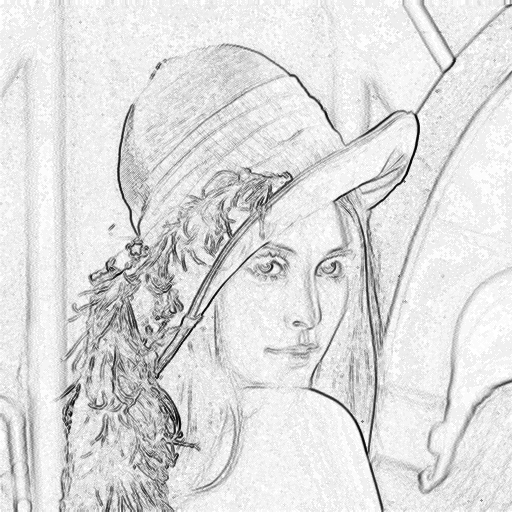
\includegraphics[width=.2\linewidth]{../figures/geninput-000b}}  &
    \fbox{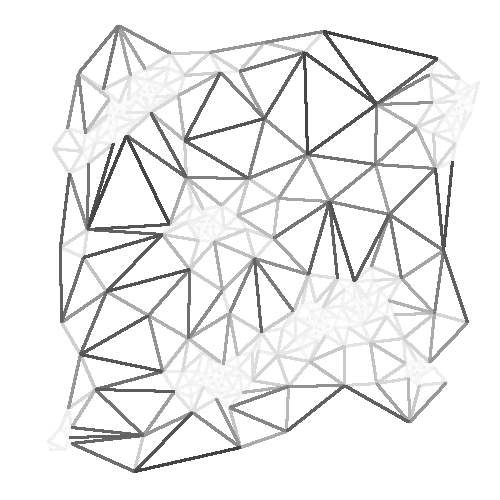
\includegraphics[width=.2\linewidth]{../figures/geninput-001b}}  &
    \fbox{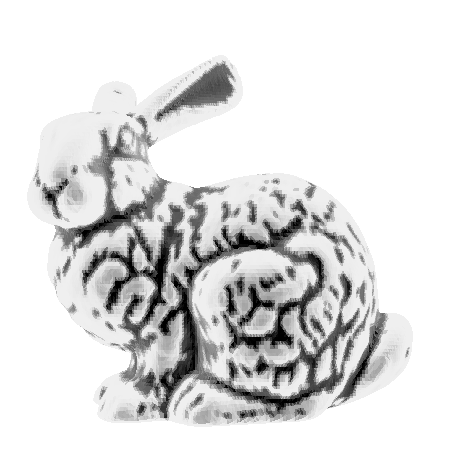
\includegraphics[width=.2\linewidth]{../figures/geninput-002b}}
    \\[5pt]
    %
    output:                                                                &
    \fbox{
\includegraphics[width=.2\linewidth]{../figures/genoutput-000}}  &
    \fbox{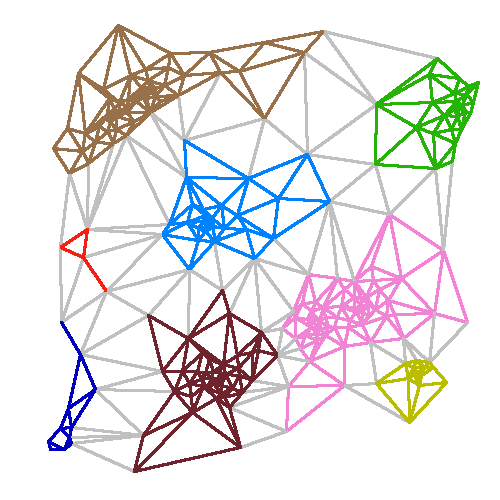
\includegraphics[width=.2\linewidth]{../figures/genoutput-001b}} &
    \fbox{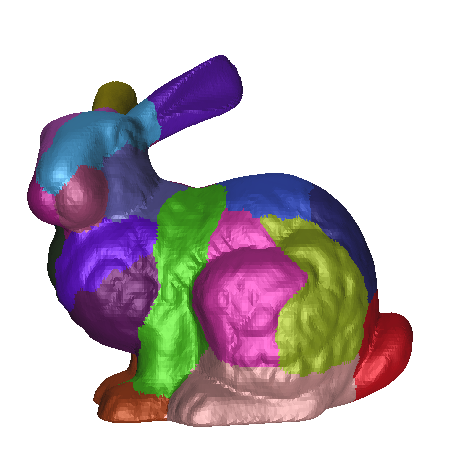
\includegraphics[width=.2\linewidth]{../figures/genoutput-002b}}
    \\
  \end{tabular}
  \bigskip

  \text{The same code run on all these inputs.}

  \caption[]{Watershed algorithm applied to three different image types.}
  \label{summary:fig:type.vs.algo}
\end{figure}

Genericity can have two different meanings depending on the people you ask. For instance, some will argue that
genericity is high level and qualifies a tool which is ``generic enough'' to handle all of his use-cases. Others will
argue that genericity is about how the code is written: generic enough to handle all the use cases possibles. Neither is
wrong. However, for the sake of comprehension we will use different words for each of these cases. A tool generic enough
to handle a lot of use-case will be called \emph{versatile}. Finally, for a tool whose aim is to provide a programming
framework to handle code of any use-case we will use \emph{generic}. In this thesis, genericity will be about code.
The~\cref{summary:fig:type.vs.algo} illustrates this result of the same generic watershed implementation applied on an
image 2D, a graph as well as a mesh.

In this chapter we present the origin of generic programming, which goes as far as~\citedate[year]{musser.1988.generic}
and how it has evolved to be integrated in the Ada programming language and then the C++ programming language.
Afterwards, it has evolved even further with the notion of \emph{concept} which completes the toolbox required to be
able to fully make use of generic programming without resorting to obscure tweaks and tools.

\begin{table}[htbp]
  \centering
  \begin{threeparttable}
    \caption[]{Genericity approaches: \pros~\& \cons}
    \begin{tabular}[width=0.8\linewidth]{l|ccccc}
      Paradigm             & TC\tnote{1} & CS\tnote{2} & E\tnote{3} & One IA\tnote{4} & EA\tnote{5} \\
      \hline
      Code Duplication     & \cmark      & \xmark      & \cmark     & \xmark          & \xmark      \\
      Code Generalization  & \xmark      & \eqmark     & \eqmark    & \cmark          & \xmark      \\
      Object-Orientation   & \eqmark     & \cmark      & \xmark     & \cmark          & \cmark      \\
      Generic Programming: &             &             &            &                 &             \\
      \quad with C++11     & \cmark      & \eqmark     & \cmark     & \cmark          & \eqmark     \\
      \quad with C++17     & \cmark      & \cmark      & \cmark     & \cmark          & \eqmark     \\
      \quad with C++20     & \cmark      & \cmark      & \cmark     & \cmark          & \cmark      \\
    \end{tabular}
    \begin{tablenotes}
      \item[1] TC: type checking.
      \item[2] CS: code simplicity.
      \item[3] E: efficiency.
      \item[4] One IA: one implementation per algorithm.
      \item[4] EA: explicit abstractions / constrained genericity.
    \end{tablenotes}
    \label{summary:table:gen.approaches}
  \end{threeparttable}
\end{table}

This chapter explores the possibilities of achieving the notion of genericity from within a library. Indeed, there are
three techniques enabling the user to write a high level algorithm once that can run on every type. They are the
\emph{code duplication} approach, the \emph{generalization} approach and the \emph{inclusion and parametric
  polymorphism} approach~\parencite{gibbons.2007.datatype}. We present in~\cref{summary:table:gen.approaches} the result
of the comparison of these approaches with regard to the features that we are interested in. We also discuss the
limitations linked to the usage of those approaches by comparing OpenCV, Scikit-Image and Pylene which make use of the
four techniques at different level to achieve different goals. Furthermore, we have identified limitations related to
the underlying data type, the structure of the domain, the optimizations and discuss the performances through a concrete
benchmark.

This chapter also explores how the notion of genericity is achieved with the programming languages. We retrace how Ada
implemented it and then how C++ permitted the expression of require-clauses (concept) as soon as C++98, even though it
was limited at that time. We explore how template metaprogramming techniques have been developed and have evolved,
alongside the C++ programming language itself, to finally reach a point in 2020 (C++20) where it is possible to write
concepts in C++.

Finally, this chapter presents the inherent limitation of C++ templates, which is that they remain in the static world
(compile time). Genericity (in the sense C++ template) does not exist in the final shipped binary to the user. The final
user, in its dynamic world (runtime) cannot use a generic (C++ code) tool. We discuss the different approaches possible
to bridge this gap between the static (compile-time) and dynamic (runtime) world.

The next chapter will make extensive use of Genericity to present the first contribution of this thesis: a taxonomy of
concepts related to Image processing.


\subsection*{Taxonomy for Image Processing: Image types and Algorithms}


In this thesis, we have pursued research into how to apply all those new generic facilities from the C++ language into
the Image processing area. This allows us to test them in a practical way on our predilection area while remembering our
past work, both success and failures in this matter. However, as we saw in the previous Chapter (Generic programming
(genericity)), birthing concepts from code is something that is done in an emerging way. Henceforth, the first work will
be to do an inventory of all existing image algorithms as well as an inventory of all image processing algorithms (both
basic and more complex) we can think of. This way, we will notice behavior patterns emerging from similar image types or
similar algorithms. We will then be able to extract behavioral patterns from this inventory in order to produce a full
taxonomy in the form of a framework of concepts related to image processing. This chapter is structured as followed.
First we will study how to extract behavioral pattern from a simple algorithm in order to refine it into one or multiple
concepts. Second we will study the theory set behind image types, their conjunctions, disjunctions. We will also produce
an inventory of image processing algorithms limited to mathematical morphologies that we will leverage for the final
step. Third, we will study the intrinsic genericity of algorithms to produce canvas taking advantage of properties
(linked to the types). Finally, we will study behavioral patterns, related to the pre-established inventory of
algorithms, in the form of a taxonomy engrave into a framework of concepts related to image processing.

In this chapter, we present that concepts are not designed after data structures but after algorithms. Indeed, a concept
consists in extracting a consistent behavioral pattern from a piece of code (algorithm) and name it to give him a
meaning. Through a simple but concrete example, we present in a didactic way how to extract concepts from an image
processing algorithm (gamma correction).

\begin{figure}[htbp]
  \centering
  \subfloat[Different versions of \emph{fill} algorithm]{
    \includegraphics[width=1.9in]{../figures/image_version}
  }%
  \hfil
  \subfloat[Specialization existing within a version]{
    \includegraphics[width=2.9in]{../figures/image_version_specialization}
  }%
  \caption[]{Set of algorithm versions (a) and its specialization existing within a version (b).}
  \label{summary:fig:image.version.vs.specialization}
\end{figure}

This chapter then proceeds to explain how, in theory, image types are related to each other. We present the set of
different image types and how algorithms exist in those sets, which introduce the notion of \emph{version} of an
algorithm. An algorithm will have different \emph{versions} for each image types set it supports. We distinguish it
(in~\cref{summary:fig:image.version.vs.specialization}) from an algorithm \emph{specialization}, the latter being the
ability to use an opportunity (related to a property) to make an optimization and increase performances.

This chapter then proceed to describe the notion how algorithm canvas which is the result flowing from the taxonomy of
image processing algorithms. Indeed, there are three main algorithm families: the pixel-wise algorithms (binary
threshold), the local algorithms (dilation) and the global algorithms (Chamfer distance transform). We focus primarily
on local algorithms and how they can all be written through the same canvas of code. Indeed, for instance, the only
difference between a dilation and an erosion is the operator (max \vs min). We then discuss ways to exploit these canvas
to possibly solve heterogeneous computing issues.

\begin{figure}[htbp]
  \centering
  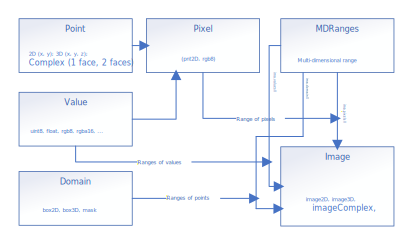
\includegraphics[width=.8\linewidth]{../figures/concepts/image}
  \caption[]{Image concept.}
  \label{summary:fig:concept.image}
\end{figure}

Finally, this chapter introduces our first main contribution: a complete taxonomy related to the image processing area.
We first introduce fundamental concepts such as \emph{point}, \emph{pixel}, \emph{domain} and \emph{image} (illustrated
in~\cref{summary:fig:concept.image}). We then motivate and introduce advanced concepts related to images and the different way
to access data (forward, backward traversing, indexing, direct access to underlying buffer, \ldots). In the end, we
introduce the concepts related to orbiting notions such as \emph{structuring element}, \emph{neighborhood} and
\emph{extension} (border management) which are necessary to be able to work with local algorithms.

The next chapter will make use of the presented concepts to introduce the second main contribution of this thesis: the
\emph{image views}.


\subsection*{Image views}


This concept of views is not new~\parencite{novak.1997.reuse} and naturally appeared in Image processing with
Milena~\parencite{geraud.2012.ipolmeeting,levillain.2010.icip} under the name of
\emph{morpher}~\parencite{levillain.2009.ismm, geraud.2012.hdr}. It was always useful to be able to project an image
through a prism that could extract specific information about it without the need to copy the underlying data buffer. In
modern days, the language C++ (20) also introduces this mechanism with the ranges~\parencite{niebler.2014.ranges}
facilities for \emph{non-owning collections}. It is named \emph{views} and allows the user to access the content of a
container (vector, map) through a prism. In Pylene, we decided to align the naming system after what was decided in
C++20 in order not to confuse the user. This way, a \texttt{transform} view in image processing will do the same thing
on an image that the transform view in the standard range library does on a container. \emph{Views} feature the
following properties: \emph{cheap to copy}, \emph{non-owner} (does not \emph{own} any data buffer), \emph{lazy
  evaluation} (accessing the value of a pixel may require computations) and \emph{composition}. When chained, the compiler
builds a \emph{tree of expressions} (or \emph{expression template} as used in many scientific computing libraries such
as Eigen~\parencite{guennebaud.2010.eigen}), thus it knows at compile-time the type of the composition and ensures a
0-overhead at evaluation. We will first motivate the usage of \emph{views} in image processing. We will then present the
main views used in image processing. Then will be discussed how image views differ from the one used in C++'s ranges and
their main properties (especially how they keep/discard the properties from the parent image) through a concrete
example: the management of border and extension policies. Finally, we will discuss the limitations of such a design.

In image processing an algorithm is naively written by taking one or several inputs' data (among which is the input
image(s)),  by performing work on this input data and then by returning the resulting data (or an error). Let us take
for example the alpha-blending example which can be implemented in naive C++ code as followed:
\begin{minted}{C++}
  void blend_inplace(const uint8_t* ima1, uint8_t* ima2, float alpha,
  int width, int height, int stride1, int stride2) {
    for (int y = 0; y < height; ++y) {
      const uint8_t* iptr = ima1 + y * stride1;
      uint8_t* optr = ima2 + y * stride2;
      for (int x = 0; x < width; ++x)
        optr[x] = iptr[x] * alpha + optr[x] * (1-alpha);
    }
  }
\end{minted}

This code has several flaws. It makes strong hypothesis about the input images: its data buffer contiguity and its shape
(2D). Let us suppose that our user now wants to restrict the algorithm to a specific region inside the image. The
maintainer would have then to provide an overload of the algorithm with one additional input argument corresponding to the
region of interest. Let us suppose that the user now wants to support manipulate 3D images. The maintainer would now
have to provide two additional overloads with an additional stride argument (one for the base algorithm, one for the
region of interest-restricted algorithm). Let us now suppose that the user only wants to manipulate the red color
channel. Now the maintainer must support and add additional overloads of the algorithm for each channel and/or color
type. The complexity increases manyfold for each kind of customization points the maintainer wants to offer to the user.
Of course, it is possible to prevent code duplication through clever usage of computer engineering techniques (code
factorization etc.) but the complexity would still leak through the API anyway. That is way the other solution is to
make the user able to perform those restriction upstream from the algorithm transparently so that the downstream
algorithm is easy to write, understand and maintain. In order to achieve this, we need to raise the abstraction level
around images by one layer so that we can work at the image level. The alpha-blending algorithm would then be written as
shown in~\cref{summary:fig:view.alphablend}.

\begin{figure}[htbp]
  \centering
  \includestandalone[mode=image, scale=0.7]{../figures/alphablend}

  \caption[]{Alpha-blending algorithm written at image level.}
  \label{summary:fig:view.alphablend}
\end{figure}

This way to express an algorithm is achieved by introducing \emph{views} to image processing. An image now is a view and
can be restricted/projected/manipulated however the user need before feeding it to an algorithm. Even the whole alpha
blending algorithm can be rewritten in terms of views entirely, as shown in~\cref{summary:fig:new.alphablend}.

\begin{figure}[htbp]
  \centering
  \begin{minipage}[b]{5.5cm}
    \includestandalone[mode=image, scale=1.0]{../figures/view_ast2}
  \end{minipage}
  \begin{minipage}[b]{5.5cm}
    \begin{minted}{c++}
    auto alphablend =
      [](auto ima1, auto ima2, float alpha) {
        return alpha * ima1 + (1 - alpha) * ima2;
      };
    \end{minted}
    \bigskip
    \bigskip
    \bigskip
  \end{minipage}
  \caption[]{Alpha-blending, generic implementation with \emph{views}, expression tree.}
  \label{summary:fig:new.alphablend}
\end{figure}

Being able to perform powerful manipulation on images before feeding them to algorithms completely nullify the initial
problem of having several overloads of the same algorithm while maintaining and documenting all the associated optional
arguments. Indeed, in order to perform the alpha-blending transformation on the base input image, all that the user must
do is:
\begin{minted}{C++}
  auto ima1, ima2 = /* ... */;
  auto ima_blended = alphablend(ima1, ima2, 0.2);
\end{minted}
If the user wants to restrict the region to be blended, or the color channel to work on, he just has to write the
following modification:
\begin{minted}{C++}
  auto roi = /* ... */;
  auto blended_roi = alphablend(view::clip(ima1, roi), view::clip(ima2, roi), 0.2);
  auto blended_red = alphablend(view::red(ima1), view::red(ima2), 0.2);
\end{minted}
The restriction is done upstream from the algorithm and propagated downstream without increasing the code complexity.
This way, view greatly increase what the user can do by writing less code.

\begin{figure}[htbp]
  \centering
  \includegraphics[scale=0.7]{../figures/pipeline}
  \caption[]{Example of a simple image processing pipeline.}
  \label{summary:fig:view.pipeline}
\end{figure}

In this chapter, we see that \emph{views are composable}. One of the most important feature in a pipeline design
(generally, in software engineering) is \emph{object composition}. It enables composing simple blocks into complex ones.
Those complex blocks can then be managed as if they were still simple blocks. In~\cref{summary:fig:view.pipeline}, we
have 3 simple image operators \emph{Image}~\(\rightarrow\)~\emph{Image} (the grayscale conversion, the sub-quantization
and the dilation). As shown in~\cref{summary:fig:view.comp}, algorithm composition would consider these 3 simple
operators as a single complex operator \emph{Image}~\(\rightarrow\)~\emph{Image} that could then be used in another even
more complex processing pipeline. Just like algorithms, image views are composable, \eg a view of the view of an image
is still an image. In~\cref{summary:fig:view.comp}, we compose the input image with a grayscale transform view and a
sub-quantization view that then feeds the dilation algorithm.

\begin{figure}[htbp]
  \centering
  \includegraphics[scale=0.7]{../figures/composition}
  \caption[]{Example of a simple image processing pipeline illustrating the difference between the composition of
    algorithms and image views.}
  \label{summary:fig:view.comp}
\end{figure}

Also, \emph{views improve usability}. The code to compose images in~\cref{summary:fig:view.comp} is almost as simple as:

\begin{minted}{c++}
auto input = imread(...);
auto A = transform(input, [](rgb16 x) -> float {
  return (x.r + x.g + x.b) / 3.f; }; );
auto MyComplexImage = transform(A, [](float x)
  -> uint8_t { return (x / 256 + .5f); }; );
\end{minted}

People familiar with functional programming may notice similarities with these languages where \emph{transform}
(\emph{map}) and \emph{filter} are sequence operators. Views use the functional paradigm and are created by functions
that take a function as argument: the operator or the predicate to apply for each pixel; we do not iterate by hand on
the image pixels.

Furthermore, \emph{views improve re-usability}. The code snippets above are simple but not very re-usable. However,
following the functional programming paradigm, it is quite easy to define new views, because some image adaptors can be
considered as \emph{high-order functions} for which we can bind some parameters, as one would do with the curry
technique~\parencite{hanus.1995.curry}. In~\cref{summary:fig:view.highorder}, we show how the primitive \emph{transform}
can be used to create a view summing two images and a view operator performing the grayscale conversion as well as the
sub-quantization which can be reused afterwards\footnote{These functions could have been written in a more generic way
  for more re-usability, but this is not the purpose here.}.

\begin{figure}
  \begin{minted}{c++}
auto operator+(Image A, Image B) {
  return transform(A, B, std::plus<>());
}
auto togray = [](Image A) { return transform(A, [](auto x)
  { return (x.r + x.g + x.b) / 3.f; };)
};
auto subquantize16to8b = [](Image A) { return transform(A,
  [](float x) { return uint8_t(x / 256 +.5f); });
};

auto input = imread(...);
auto MyComplexImage = subquantize16to8b(togray(A));
  \end{minted}

  \caption[]{Using high-order primitive views to create custom view operators.}
  \label{summary:fig:view.highorder}
\end{figure}

In addition, \emph{views are lazy computed}. Because the operation is recorded within the image view, this new image
type allows fundamental image types to be mixed with algorithms. In~\cref{fig:view.highorder}, the creation of views
does not involve any computation in itself but rather delays the computation until the expression \texttt{v(p)} is
invoked. Because views can be composed, the evaluation can be delayed quite far. Image adaptors are \emph{template
  expressions}~\parencite{veldhuizen.1995.expression, veldhuizen.2000.blitz} as they record the \emph{expression} used to
generate the image as a template parameter. A view actually represents an expression tree (\cref{fig:new.alphablend}).

Also, \emph{views are efficient}. With a classical design, each operation of the pipeline is implemented on ``its own''.
Each operation requires memory to be allocated for the output image and also, each operation requires that the image is
fully traversed. This design is simple, flexible, composable, but is not memory efficient nor computation efficient.
With the lazy evaluation approach, the image is traversed only once (when the dilation is applied) which has two
benefits. First, there are no intermediate images which is very memory efficient. Second, traversing the image is faster
thanks to a better memory cache usage, and performs an optimal selective traversal. Indeed, in our example
(\cref{summary:fig:view.pipeline}), processing a RGB16 pixel from the dilation algorithm directly converts it in
grayscale, then sub-quantize it to 8-bits, and finally makes it available for the dilation algorithm. It acts \emph{as
  if} we were writing an optimal operator that would combine all these operations. This approach is somewhat related to
the kernel-fusing operations available in some HPC specifications~\parencite{openvx.2019} but views-fusion is optimized
by the C++ compiler only~\parencite{brown.2018.ranges}. The selective aspect intervenes when a region of interest is
selected at one point in the processing pipeline. Indeed, the entirety of the pipeline is then executed only on the
region of interest, even if this selection happens only at the very end of the processing pipeline.

Finally, \emph{views improve the productivity}. All point-wise image processing algorithms can (and should) be rewritten
intuitively by using a one-liner view. The \emph{transform} views is the key enabling that point. This implies that
there exist a new abstraction level available to the practitioner when prototyping their algorithm. The time spent
implementing features is reduced, thus the feedback-loop time is reduced too. This naturally brings productivity gain to
the practitioner.


\subsection*{A bridge between the static world and the dynamic world}


In the programming world, there are three main families of programming
language~\parencite{prechelt.2000.comparison}. There are (i) \emph{compiled} programming languages, such as C, C++, Rust
or Go, (ii) \emph{interpreted} programming languages, such as Python, PHP, Lisp or Javascript, and (iii) hybrid
programming languages, such as Java or C\#. The latter have a fast compilation pass that compiles the source code into
an intermediate bytecode. Then, this bytecode is interpreted via an interpreter on the host (runner) machine.

\begin{figure}[htbp]
  \centering
  \includegraphics[width=.6\linewidth]{../figures/type-erased_buffer}
  \caption[]{Bridge from Python to C++ via Pybind11 and a type-erased C++ class.}
  \label{summary:fig:type-erased.buffer}
\end{figure}

In this chapter, we design many solutions to solve several kinds of issues related to the bridge between the static and
the dynamic world. We present our hybrid solution that is able to make our C++ templated library (static) available from
Python (dynamic). We discuss several ways of achieving this feat, their \pros and their \cons. Also, we introduce a new
abstraction layer, the value-set, which is a standard way to manipulate an underlying image value usable when
implementing image processing algorithms. This new abstraction layer enables the user to inject code from Python-side
into already-complied C++ routines. However, layering one abstraction layer after another, or even calling Python code
does come with performance cost. This is why we have run a benchmark to outline the cost of our solutions. This
benchmark compares the four version of our stretch algorithm whose implementation and usage are detailed in the chapter.
The result is shown in~\cref{summary:table:static.dynamic.perfs}.

\begin{table}[htbp]
  \footnotesize
  \centering
  \begin{tabular}{l|ccc}
    \toprule
    Dispatch type                                               &
    Compute Time                                                &
    \(\Delta{}\)Compute Time
    \\ \midrule Native value-set with native C++ value-type (baseline)
                                                                & \(0.0093s\) & \(0\) \\
    Value-set with virtual dispatch with native C++ value-type  &
    \(0.1213s\)                                                 &
    \(\times 13\)
    \\
    Value-set with virtual dispatch with C++ type-erased values &
    \(1.0738s\)                                                 &
    \(\times 115\)
    \\
    Injected Python value-set with native C++ value-type        &
    \(21.5444s\)                                                &
    \(\times 2316\)
    \\
    \bottomrule
  \end{tabular}
  \caption[]{Benchmarks of all our version of the stretch algorithm.}
  \label{summary:table:static.dynamic.perfs}
\end{table}

This benchmark shows that each time an abstraction layer is added on top of the baseline, the user must expect a
\(10\times\) slowness factor in his code performance. Also, calling Python code is immensely slower (\(2300\times\) !)
than the baseline. This renews the interest there is to recompile the templated C++ library with an additional known
type than injecting it from Python for code taking long time to execute. Being able to inject Python code ease
prototyping and increase the speed at which the user can write his code. However, the benchmark shows that this is not a
viable solution once the prototype needs to scale to a production environment.

\paragraph{Continuation: JIT-based solutions, \pros and \cons}

Our hybrid solution certainly has advantages, but the huge disadvantage is the slowness of injecting our own types from
the Python side. There exists another solution that this thesis did not have the opportunity to study in-depth. This
solution is based on a known technology: the Just-In-Time (JIT) compilation which has been previously illustrated
in~\cref{fig:static.dynamic.dynamic.pipeline} (and which itself is based on the notion of generative
programming~\parencite{czarnecki.2000.generative}). Library such as AsmJit~\parencite{kobalicek.2011.asmjit} are able to
emit machine code directly by making call in C++ code. Indeed, it is a technology already used by interpreted languages
such as Java or PHP to generate on-the-fly native and optimized machine code for the section of the source code that is
considered ``hot'' by the interpreter. A source code is ``hot'' when it is executed a lot: the end-user would gain
paying the compilation time once to have this code executed faster several times later on. When applying this strategy
to our problematic, it would mean that the user must be able to compile native machine code from the templated generic
C++ code by injected the requested type when it is used. Such an operation shift heavily the burden on the user, and it
is well-known that compiling C++ code is notably \emph{complicated} and \emph{slow}. In addition, the library needs to
be able to auto-generate Python binding once the C++ code is compiled. There are several solutions to reach this point.

The first solution is to basically use system call to the compilers to actually \emph{compile} C++ code once the
templated types are known and explicitly instantiated in the source code. This solution requires careful code-generation
design and that the user actually possess a compiler on his computer. Furthermore, the user must resolve all the
library dependencies, such as \emph{freeimage} for IO etc. This solution was engineered in the VCSN
library~\parencite{demaille.2013.vcsn}. Indeed, each time the user declared a new automaton in his Jupyter notebook,
corresponding source code is compiled in the background and then cached. It is a very perilous solution to implement
when the final execution environment (OS, installed software) is not well-known in advance. Nowadays, the issue may be
lesser, however, it still requires to maintain both the library and the container solution to use it (Docker).

The second solution is to use Cython~\parencite{behnel.2010.cython}. It is a transpiling infrastructure which transform
a Python source code directly into C-language source code so that it can be compiled by a standard C compiler just by
linking against the Python/C API. This remove the burden of writing the careful code-generation routine, system-calls
to the C++ compiler and removes the need to resolve all the dependencies. This infrastructure takes care of everything
for the user. Also, by transpiling it into C code, it is faster because a C compiler is faster than a C++ compiler.
Cython even support C++ template code~\parencite{behnel.2022.cython-template} which is mandatory for our use-case.

The third solution consists in relying on recent projects that are all relying on the LLVM infrastructure. We can
notably note AutoWIG~\parencite{fernique.2018.autowig}, Cppyy~\parencite{wimtlplavrijsen.2016.cppyy},
Xeus-cling~\parencite{quantstack.2021.xeus-cling} and Pythran~\parencite{guelton.2015.pythran}. AutoWIG has in-house
code based on LLVM/Clang to parse C++ code in order to generate and compile a Swig Python binding using the Mako
templating engine. AutoWIG, coupled with Cython would permit the user to, for instance, generate C code related to a
custom Python structure. Then a simple call to AutoWIG will parse the C code and inject it into the C++ library to
generate the appropriate bindings for the user. As for Cppyy, it is based on LLVM/Cling, a C++ interpreter, and can
directly interpret C++ code from a Python string. This enables injecting custom types easily, be they in Python code
(transpiled with Cython) or C++ code (directly interpreted by Cling). Afterwards, the infrastructure generates the
appropriate binding from the templated C++ library for the injected type. Xeus-cling is a ready-to-use Jupyter kernel
and allow the usage of C++ code directly from within a notebook. This completely bypass the need of a Python binding in
the first place and allow the user to use the library from within the notebook as if he was using a Python library.
Finally, Pythran is an ahead of time compiler for a subset of the Python language, with a focus on scientific computing.
It takes a Python modle annotated with a few interface descriptions and turns it into a native Python module with the
same interface, but hopefully faster. Pythran takes advantages of multicore and SIMD instructions to turns its subset of
the Python language into heavily templated C++ code instantiated for particular optimized types. All those
infrastructures, however, come with a hefty cost in terms of binary size. Indeed, a C++ compiler is not small and
embarking it alongside the image processing library can easily impact greatly the final binary. Without the LLVM
infrastructure the binary may weight around 3MB. With the LLVM infrastructure, the binary weight at the bare minimum
50MB. Also, these solutions may not be immediately faster. Indeed, when prototyping back and forth with a variety of
types, the user may not be eager to wait for long compilations times each time he is testing with a new iteration of his
work. Despite those facts, those solutions offers great avenue of research for the future and the author is eager to
explore them.


\subsection*{Conclusion}


The work presented in this thesis by the author followed a very clear narrative arc. The emphasis was first shown on
presenting what is the notion of generic programming (genericity), its story and how anyone can relate in his day-to-day
life, especially when applied to image processing. Genericity is a 4-decades years old notion that has evolved and found
usage in very modern areas of our society. Indeed, image processing is widely used to build modern applications used all
around the world. However, it was demonstrated how difficult it can be to implement solutions relying on genericity.
Indeed, there is a rule of three tying genericity, performance and ease of use. The rule states that one can only have
two of those items by sacrificing the third one. If one wants to be generic and efficient, then the naive solution will
be very complex to use with lots of parameters. If one wants a solution to be generic and easy to use, then it will be
not very efficient by default. Finally, if one wants a solution to be easy to use and efficient then it will not be very
generic. In this thesis, we try to demonstrate how to break this rule in three steps.

The first step, illustrated in the chapter \emph{Taxonomy for Image Processing}, was to make an inventory of image types
and families as well as different image processing algorithms. The aim was to produce a comprehensive taxonomy of types
(pixel, image, structuring elements, \ldots) and algorithms related to image processing in order to be able to write
concepts (in the sense of C++ concepts). This first step delimits the perimeter of what the author means by
\emph{genericity}. From this starting point, it becomes easier to write image processing algorithms, just by relying on
those concepts. Furthermore, different concepts exist to enable algorithm implementers to leverage properties
(structuring elements' decomposability, image's buffer contiguous, \ldots) in order to achieve maximum performance.

At this point, we are still reasoning at a low level (pixel) which generates the need to design an abstraction layer in
order to enable fast prototyping for simple operations while guarantying very small memory footprint and near-zero
performance impact. For this reason, we expand the concept of \emph{views} from the C++ standard (2020) to images and
design what the notion of \emph{image view}. We also make the design choice to have cheap-to-copy image (shared data
buffer) by default in order to merge concrete image and views from the user point of view. The lazy-evaluation, that
systematically happens when using views allows performance gain when clipping larges images. In the case where the whole
image is processed, we were able to still retain very satisfactory performance that remain stable. Also, we show through
concrete use-case, such as pixel-wise algorithm and border management how the usage of views simplify greatly how to
write more complex image processing algorithms that are efficient by default. We finally show the limitations of this
approach, with a particular focus on the speed of traversing an image, which a mandatory use-case we must get right.

Finally, this thesis focused its attention on how it is possible to distribute this software to the image processing
community which is mainly working with Python. The last work concentrates its efforts on finding the best way to design
a static (compile-time, templated C++) --- dynamic (runtime, Python notebook) bridge to bring those notions (concepts
and views) to the practitioner, efficiently. This last work explores this dilemma and offers to address it with one
hybrid solution whose design is explained in-depth. This hybrid solution rely on a type-erased type which offers
compatibility with a \emph{NumPy.array}~\parencite{harris.2020.numpy}. It is then able to cast itself inside an \(n
\times n\) dispatcher (dimension and underlying type) into an optimized concrete templated C++ type. This solution also
explain how to write very simply the glue code enabling already-existing algorithms (in C++) to be exposed in Python
thanks to a dispatch mechanic heavily inspired from the C++ standard (\texttt{std::visit}, \texttt{std::variant}). The
aim of this solution was to regroup at a single place in the code all the supported types into the dispatchers for
maintenance purpose as well as demanding minimal work from algorithm implementer to expose their algorithms, all this
while keeping the native performance. Indeed, no superfluous copy is performed thanks to \emph{pybind11}'s
\emph{type-caster} facility, and one cast is done from the type-erased type to the native one. All the work that is done
in the algorithm is performed on native optimized type. Finally, this solution offers a way to inject custom Python
types into the library for prototyping purpose, thanks to a new abstraction layer, at the cost of heavy performance
loss. The downside of this solution is obviously the code bloat with the resulting binary size exploding exponentially
with the number of supported types multiplied by the number of algorithms multiplied by the number of additional
supported data (structuring elements, label map, etc.)

We conclude this thesis by offering new avenue of research around the Just-In-Time (JIT) compilation area to further
improve the bridge between the static and the dynamic world. The author thinks that this avenue is worth exploring,
especially with the already promising existing tools (Xeus-cling, Cppyy, Cython, AutoWIG, Pythran) in order to solve the
code bloat issue. Indeed, we would only compile what the user need, but the entry price may be to statically link a C++
interpreter (LLVM/cling?) into the binary which in itself would greatly bloat it. It may be possible, however, to rely
on the user's system-wide infrastructure so that the maintenance does not distribute a whole C++ interpreter/compiler
alongside his image processing library binary. This is still a new area of research and the author would very much want
to delve into it to study what is possible to achieve as of today with those tools for the image processing community.
